\documentclass[a4paper]{scrartcl}

\usepackage[utf8]{inputenc}
\usepackage[french]{babel}
\usepackage{graphicx}
\usepackage[cm]{fullpage}
\usepackage{multirow}
\usepackage[bookmarksnumbered,colorlinks,backref, bookmarks, breaklinks, linktocpage, pdfstartview=FitH]{hyperref}
\hypersetup{
    bookmarks=true,
    unicode=false,
    pdftoolbar=true,
    pdfmenubar=true,
    pdffitwindow=false,
    pdfstartview={FitH},
    pdftitle={Test de recrutement},
    pdfauthor={Nicolas Dubois - ndubois@amg-dev.fr},
    pdfsubject={Exercice},
    pdfkeywords={PPO, PHP, TDD},
    pdfnewwindow=true,
    colorlinks=false,
    linkcolor=red,
    citecolor=green,
    filecolor=magenta,
    urlcolor=cyan
}

% Nice URLs:
\usepackage{url}\urlstyle{sf}

\titlehead{
\begin{center}

\begin{tabular}{p{12cm}r}
\sf AMG Développement - GPdis/P\^ole e-commerce 
&
\multirow{4}{*}{

\includegraphics[width=35mm]{../images/amg-developpement-logo.png}
} \\

\sf 13 avenue du Fontréal & \\
\sf BP 72 172 & \\
\sf 31621 EUROCENTRE CEDEX & \\

\end{tabular}
\end{center}
}
\subject{\titlefont Test de recrutement}
\title{Exercice}
\author{\titlefont Nicolas Dubois $\cdot$ ndubois@amg-dev.fr}
\date{\sf Mardi 1 février 2011}
\publishers{\sf Version 1.0}

\begin{document}

\maketitle

%\tableofcontents

\section{Définition}

\begin{quotation}
En théorie des ensembles, un ensemble désigne intuitivement une collection d’objets (les éléments de l'ensemble), 
« une multitude qui peut être comprise comme un tout » (au sens d'omnis). Pour notre exercice, les objets seront des nombres entiers distincts.
\end{quotation}

La figure \ref{fig:set} présente un exemple d'ensemble contenant les entiers suivants : $\{ 2, 3, 6, 7, 14 \}$.

\begin{figure}[ht!]
\begin{center}
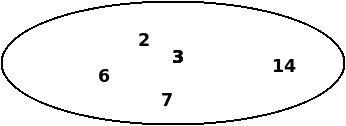
\includegraphics[width=5cm]{../images/Set.png}
\end{center}
\caption{Exemple d'ensemble}
\label{fig:set}
\end{figure}

\section{Modélisation objet}

On se propose de modéliser un ensemble par une classe abstraite et une implémentation simple, à l'aide 
d'un tableau qui contiendra les éléments. La figure \ref{fig:uml-diagram} montre les 3 classes à implémenter. 

\begin{figure}[ht!]
\begin{center}
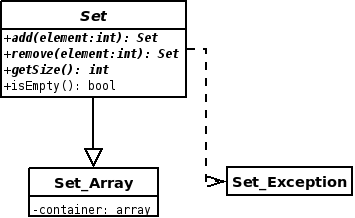
\includegraphics[width=8cm]{../images/UML-Diagram.png}
\end{center}
\caption{Diagramme UML}
\label{fig:uml-diagram}
\end{figure}

Les méthodes en gras sont des méthodes abstraites. Voici le comportement attendu par les 4 méthodes de l'objet
\emph{Set} :

\begin{quote}
\begin{description}
\item[add()] : ajoute\footnote{Attention, l'ensemble ne contient que des entiers distincts. Donc si l'élément existe déjà, 
	il ne doit pas appara\^i tre en double.} l'élément passé en paramètre à l'ensemble.
\item[remove()] : supprime l'élément passé en paramètre de l'ensemble. Si l'élément n'existe pas dans le tableau, 
	l'exception Set\_Exception est déclenchée.
\item[getSize()] : retourne le cardinal de l'ensemble (\emph{i.e.}, le nombre d'élément contenu dans l'ensemble).
\item[isEmpty()] : retourne un booléen pour dire si l'ensemble est vide ou non.
\end{description}
\end{quote}

De plus, les méthodes \emph{add()} et \emph{remove()} de l'objet \emph{Set} devront permettre le cha\^inage de méthodes (\verb!Fluent Interface!).

\section{Approche}

Pour le développement de ces 3 classes, nous utiliserons une méthode de développement dirigée par les tests (TDD). Dans le 
répertoire \emph{tests/}, vous pourrez lancer le script \verb![shell] sh run_tests.sh! pour exécuter l'ensemble des tests. 
À l'issue du test, l'ensemble des 4 tests (14 assertions) doivent \^etre correctement passés.

\section{Ressources}

Toutes les ressources sont autorisés pour la résolution du problème.

\end{document}
